\section{Entwurf des zentralen Systems}\label{l:entwurf}

\begin{figure}[htb]
\begin{center}
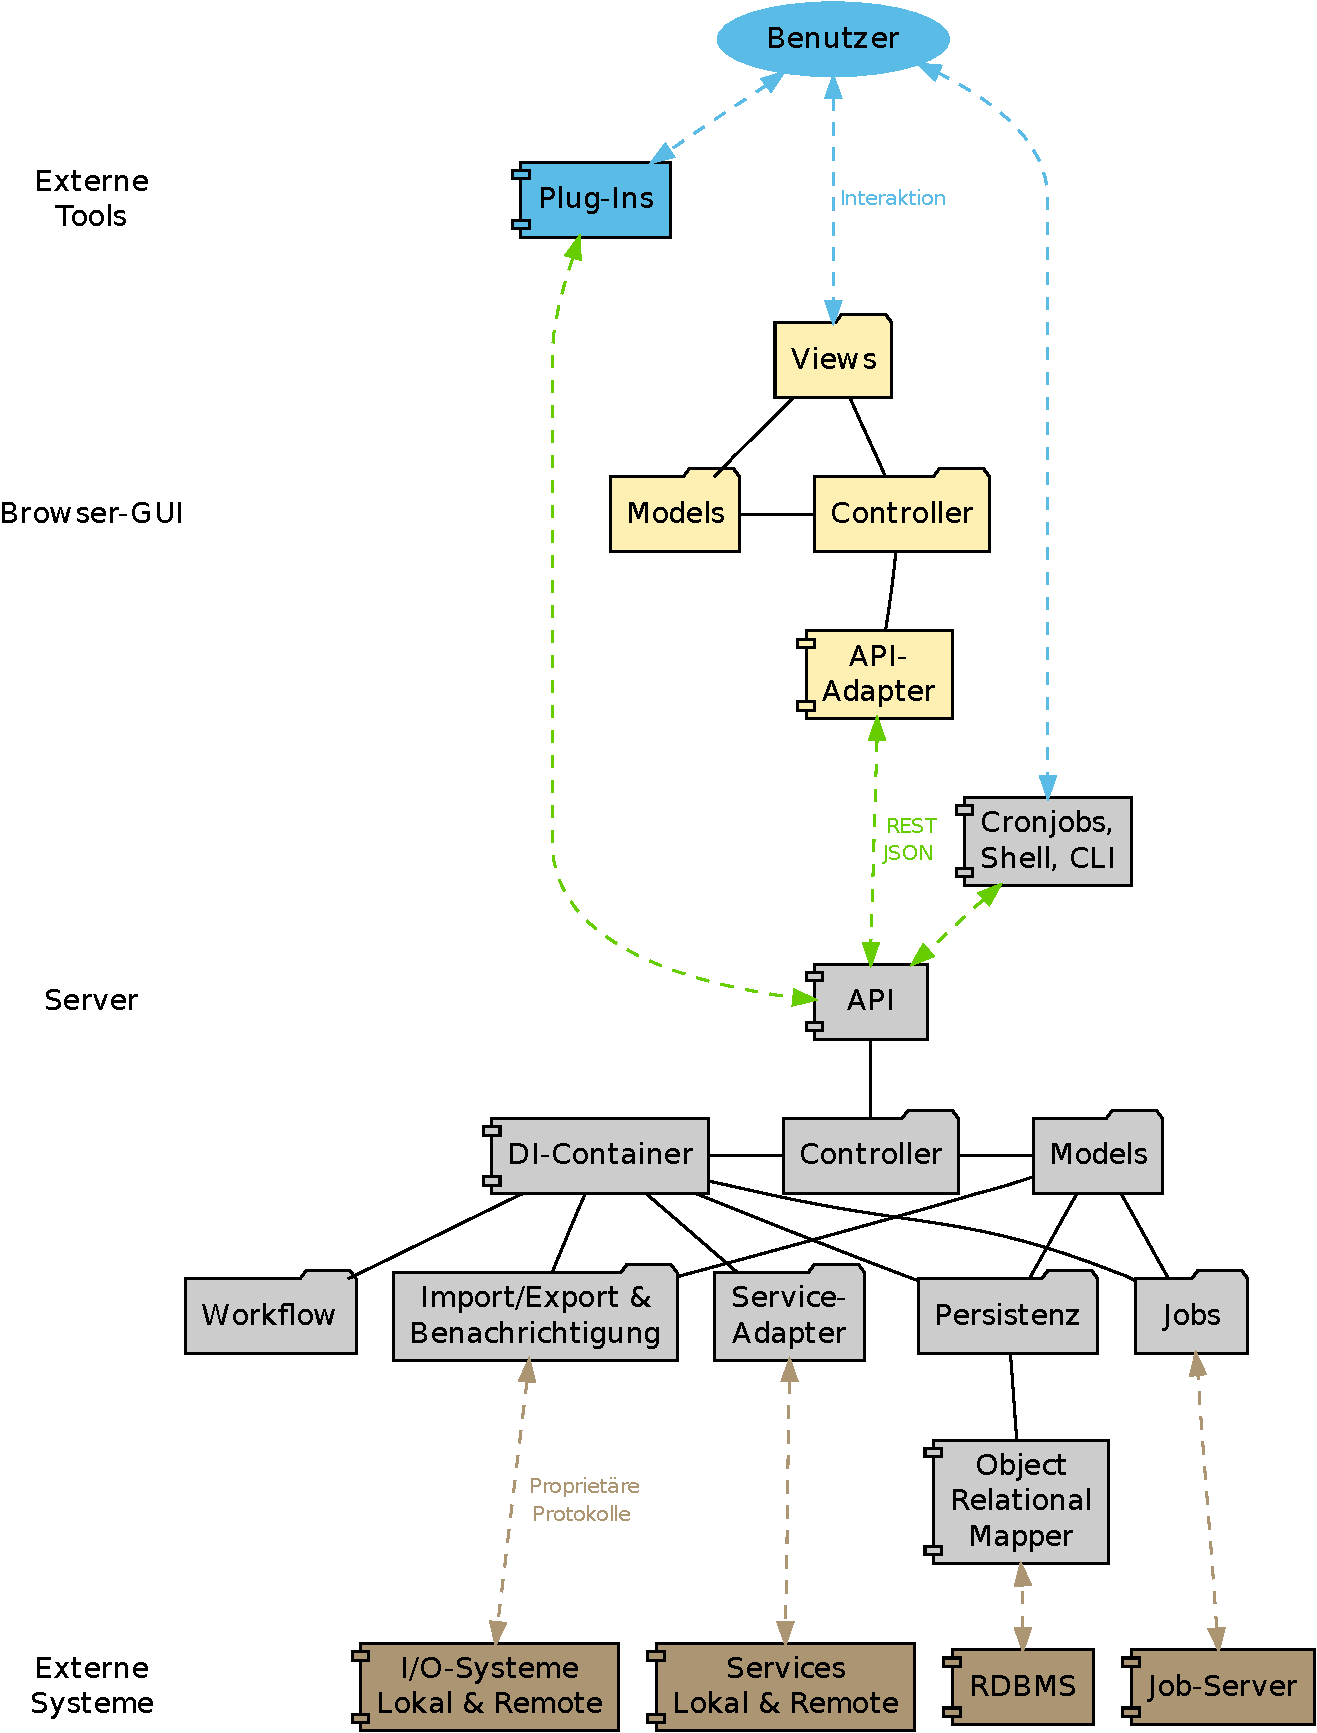
\includegraphics[width=0.6\textwidth]{media/komponenten.pdf}
\end{center}
\caption{Komponententen des zentralen Systems}
\label{chart:komponenten}
\end{figure}

Im vorigen Abschnitt~\ref{l:konzeption}~(S.\pageref{l:konzeption}~ff.) wurde eine Anwendung konzipiert, die das gesamte Spektrum der Anforderungen abdeckt, die in den vorangegangenen Abschnitten beschrieben wurden. In diesem Abschnitt werden die Komponenten beschrieben, die zur Erfüllung der wichtigsten Anforderungen benötigt werden. 

Abbildung~\ref{chart:komponenten} liefert einen Überblick über die in den folgenden Abschnitten beschriebenen Komponenten des Systems. \emph{Blau} eingezeichnet sind der Endanwender und externe Benutzer-Werkzeuge wie z.B. Plug-Ins und Software von Drittanbietern. \emph{Gelb} eingezeichnet sind die Komponenten des browserbasierten GUI. \emph{Grau} eingezeichnet sind die Komponenten des Servers. \emph{Braun} eingezeichnet sind (aus Sicht des Servers) externe Dienste, die durch diesen angebunden werden. \emph{Gestrichelte Linien} zeigen Kommunikationsverbindung zwischen Komponenten über Schnittstellen. \emph{Durchgezogene Linien} zeigen Verbindungungen innerhalb eines Systems. 

Der zentrale Bestandteil der Anwendung ist der Server, mit dem verschiedene GUIs über Schnittstellen kommunzieren. Das wichtigsten GUI ist das browserbasierte Interface, da hiermit alle Mitarbeiter arbeiten, dessen Gestaltung in Abschnitt~\ref{l:entwurf-gui}~(S.\pageref{l:entwurf-gui}) und Anbindung an den Server in Abschnitt~\ref{l:anbindung-gui}~(S.\pageref{l:anbindung-gui}) beschrieben wird. Abschnitt~\ref{l:entwurf-server}~(S.\pageref{l:entwurf-server}) beschreibt die Komponenten des Servers. Abschließend wird in Abschnitt~\ref{l:domänenmodell}~(S.\pageref{l:domänenmodell}) das Domänenmodell vorgestellt, das allen Teilen der Anwendung zu grunde liegt.

\subsection{Entwurf eines browserbasierten GUI}\label{l:entwurf-gui}

Das browserbasierte GUI der Anwendung ist der wichtigste Zugang zum System, da es von allen Mitarbeiter zu irgendeinem Zeitpunkt verwendet wird. Die Zeit, die der Einzelne damit verbringt kann sich je nach Rolle stark unterscheiden. Neben den sehr unterschiedlichen Anforderungen and das GUI sind die Benutzer auch technisch sehr unterschiedlich stark versiert, wie in den Personas in Abschnitt~\ref{l:personas}~(S.\pageref{l:personas}~ff.) gezeigt wurde. Diesen Umständen muss bei der Gestaltung eines GUI Rechnung getragen werden. In Anlehnung an \cite{nielsen} wurden für den Entwurf der browserbasierten GUI folgende Leitlinien gewählt:

\begin{enumerate}\itemsep -5pt
\item{Das wichtigste zuerst: Die aktuelle Aufgabe soll immer im Fokus der Darstellung liegen.}
\item{Schnell zum Ziel: Alle Aufgaben müssen leicht und umkompliziert durchführbar sein.}
\item{Nicht ablenken: Veränderungen in der Darstellung, z.B. durch Benachrichtigungen, lenken ab und müssen deswegen so gestaltet sein, dass diese sich nach den Präferenzen des Nutzers richten.}
\item{Hilfe nur einen Klick entfernt: Das Hilfesystem muss kontextsensitiv verfügbar sein und ist eine Kernfunktion der Anwendung}
\end{enumerate}

Da die Anwendung von allen Benutzern gerne verwendet werden soll und vor allem die Usability und die Zeitersparnis ein wichtiger Punkt sind, wie man auch skeptische Mitarbeiter überzeugen kann, mit ihren alten Gewohnheiten zu brechen, ist die Beachtung dieser Grundsätze essentiell. Funktionalitäten, die nur von wenigen gebraucht werden, sollten, wenn überhaupt, optional einblendbar sein. Die Konzeption des Systems ermöglicht es leicht, zusätzliche Anwendungen für besondere Benutzergruppen zu schaffen, z.B. Plug-Ins für die speziellen Werkzeuge einzelner Mitarbeiter. Für diese \typoquotes{Power-User} ist dieser Weg meistens der bessere Weg.

\begin{table}
\begin{center}
\begin{tabular}{@{}l c c c c c c c}
& \textbf{Eva} & \textbf{Lotte} & \textbf{Torsten} &  \textbf{Jorinde} & \textbf{Jan} & \textbf{Arthur} & \textbf{Markus}\\
{\small Operation (vgl.~\ref{l:workflow})} & {\small Konz.} & {\small Des.} & {\small Texter} & {\small Übersetz.} & {\small Prod.} & {\small Projektl.} & {\small Kunde}\\
\hline\\[-1.5ex]
Definieren         & \HarveyFull      & \HarveyQuarter   & \HarveyEmpty    & \HarveyEmpty    & \HarveyEmpty   & \HarveyEmpty     & \HarveyEmpty \\
Schreiben          & \HarveyQuarter   & \HarveyEmpty     & \HarveyFull     & \HarveyFull     & \HarveyEmpty   & \HarveyEmpty     & \HarveyEmpty \\
Korrektur          & \HarveyEmpty     & \HarveyEmpty     & \HarveyHalf     & \HarveyHalf     & \HarveyEmpty   & \HarveyQuarter   & \HarveyQuarter \\
Qualitätskontrolle & \HarveyQuarter   & \HarveyEmpty     & \HarveyEmpty    & \HarveyEmpty    & \HarveyEmpty   & \HarveyFull      & \HarveyHalf \\
Freigabe           & \HarveyEmpty     & \HarveyEmpty     & \HarveyEmpty    & \HarveyEmpty    & \HarveyEmpty   & \HarveyQuarter   & \HarveyQuarter \\
Veröffentlichung   & \HarveyEmpty     & \HarveyEmpty     & \HarveyEmpty    & \HarveyEmpty    & \HarveyQuarter & \HarveyEmpty     & \HarveyEmpty \\
\end{tabular}
\caption{Umfang und Häufigkeit der Benutzung des browserbasierten GUIs bezogen auf die durchgeführten Operation}
\label{table:webgui-usage-by-persona}
\end{center}
\end{table}

Anhand der Personas lässt sich ermitteln, wer und in welchem Umfang das browserbasiert GUI verwenden wird. Tabelle~\ref{table:webgui-usage-by-persona}~(S.\pageref{table:webgui-usage-by-persona}) zeigt in der Übersicht, welche Operationen besonders bei der Entwicklung des GUIs beachtet werden müssen. Besonders viel Zeit werden von Konzeptern und von den Mitarbeiter, die die Inhalte erstellen, kontrollieren und freigeben im GUI verbracht, da diese Tätigkeiten bezogen auf die einzelnen Texte des Produktes sehr arbeitsintensiv sind.

\bigskip

Die folgenden Wireframes zeigend dementsprechend die wichtigsten Ansichten des GUIs.

\subsubsection{Aufbau des GUIs}

\begin{center}
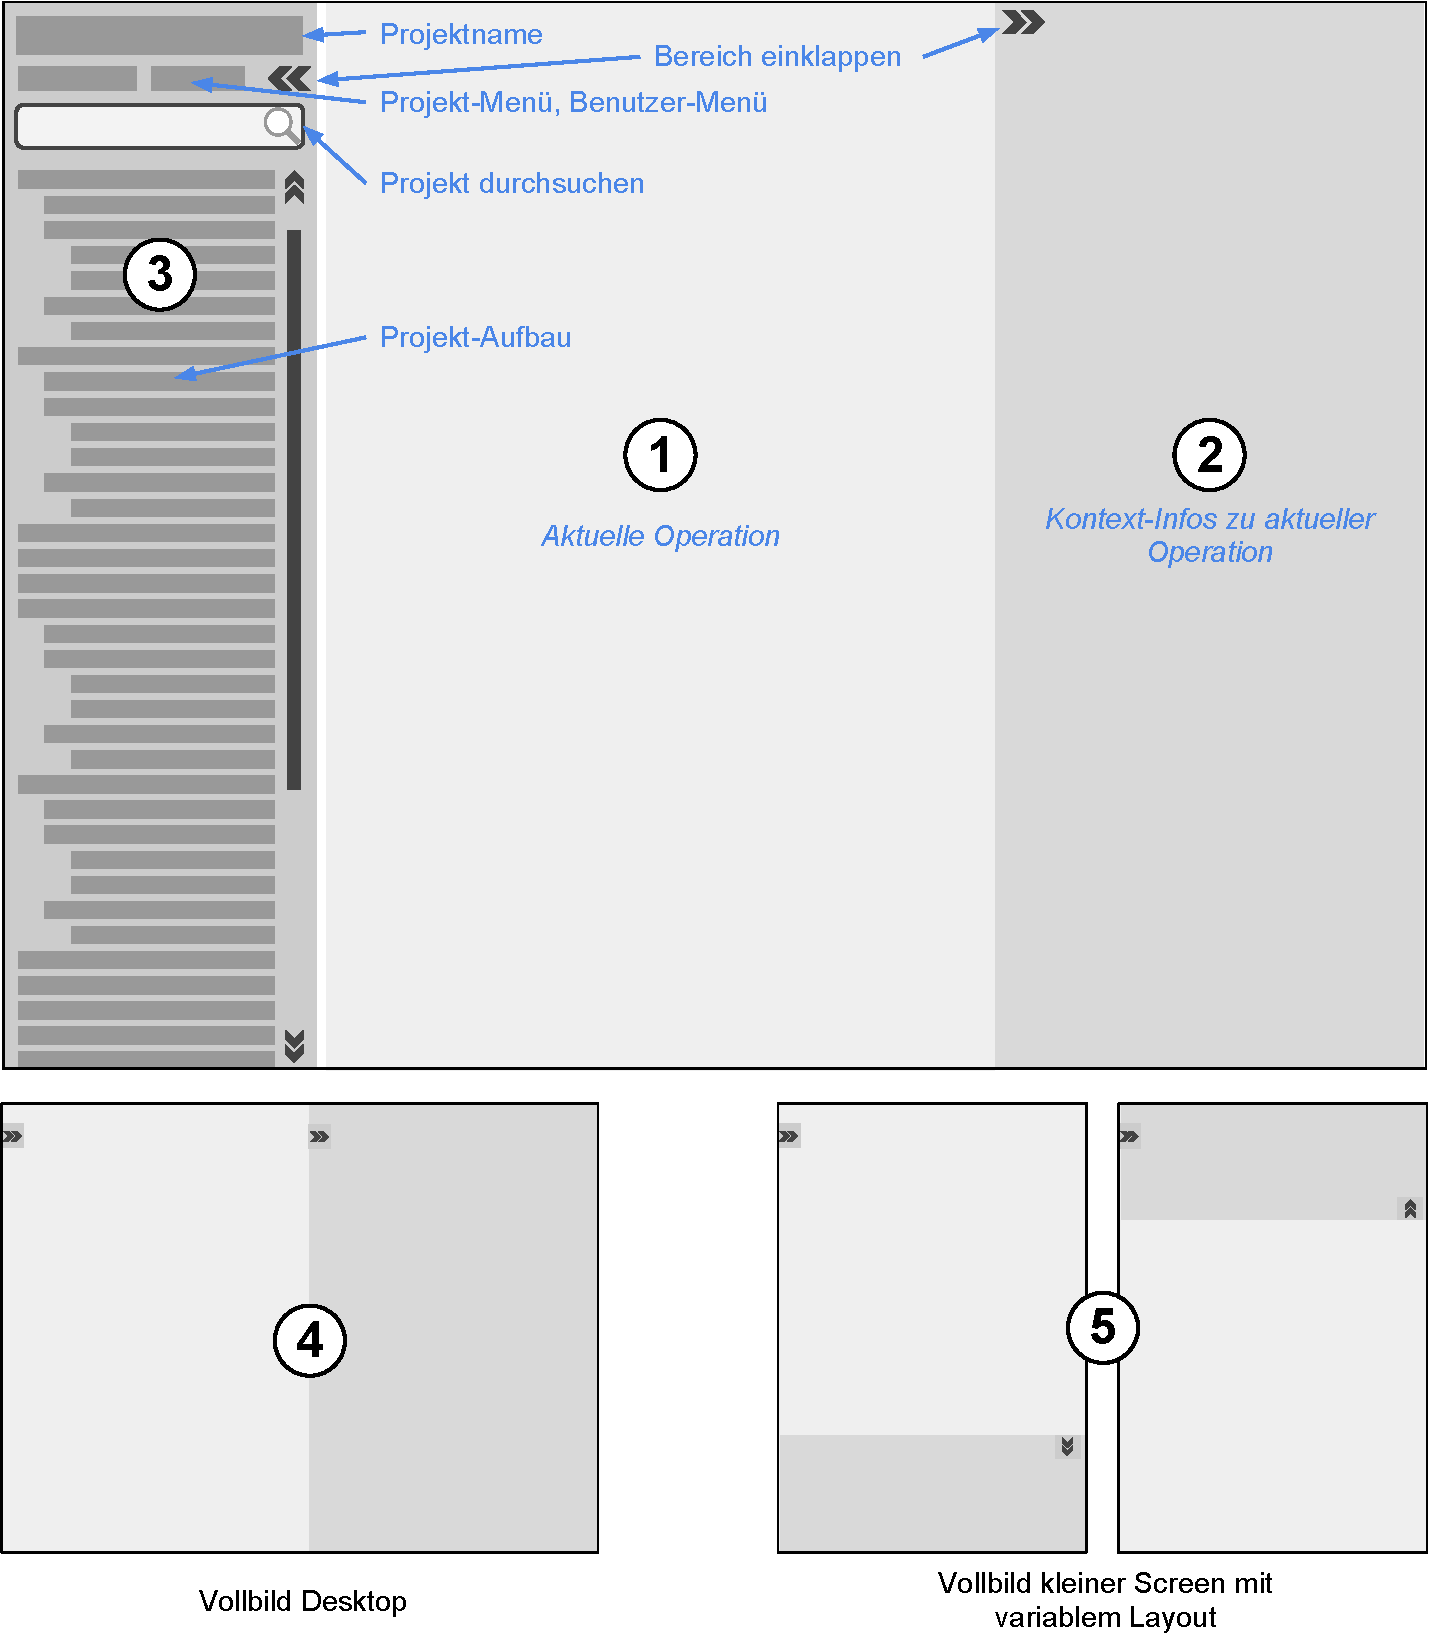
\includegraphics[width=0.95\textwidth]{media/GUIAufbau.pdf}
\captionof{figure}{Aufbau des browserbasierten GUIs}\label{chart:gui-aufbau}
\end{center}

Abbildung~\ref{chart:gui-aufbau} zeigt den Grundaufbau des GUIs. Zentraler Bereich ist die Darstellung der \emph{aktuellen Operation} \ball{1} mit den zugehörigen \emph{Kontext-Informationen} \ball{2}. Auf der linke Seite findet sich eine Spalte über die im Projekt navigiert werden kann \ball{3}. Um den Fokus auf die aktuelle Aufgaben zu verbessern sind die Kontext-Information und die Projektspalte ausblendbar \ball{4}. Das gesamte Layout passt sich flexibel an verschiedene Bildschirmgrößen und -formate an, zusätzlich kann die Position der Kontext-Information an die eigenen Vorlieben angepasst werden \ball{5}.

Die Projekt-Spalte \ball{3} bietet direkten Zugang zu allen Teilen des aktiven Projekts. Die Projektstruktur wird mit einem Navigationsbaum dargestellt, über den direkt zu den jeweiligen Abschnitten gesprungen werden kann. Über das Suchfeld lässen sich die Einträge im Baum filtern. In der Spalte befindet sich oben zur Orientierung der Names des aktiven Projektes. Über das ausklappbare Projektmenü gelangt man Teilen der Anwendung, die nicht direkt über die Texte erreichbar sind, z.B. Projektauswahl, Mitarbeiterverwaltung, Export. Über das ausklappbare Benutzermenü kann man sich ausloggen, sein Profil bearbeiten und persönliche Einstellungen anpassen.

\subsubsection{Definieren des Produktes}\label{l:gui-definition}

\begin{center}
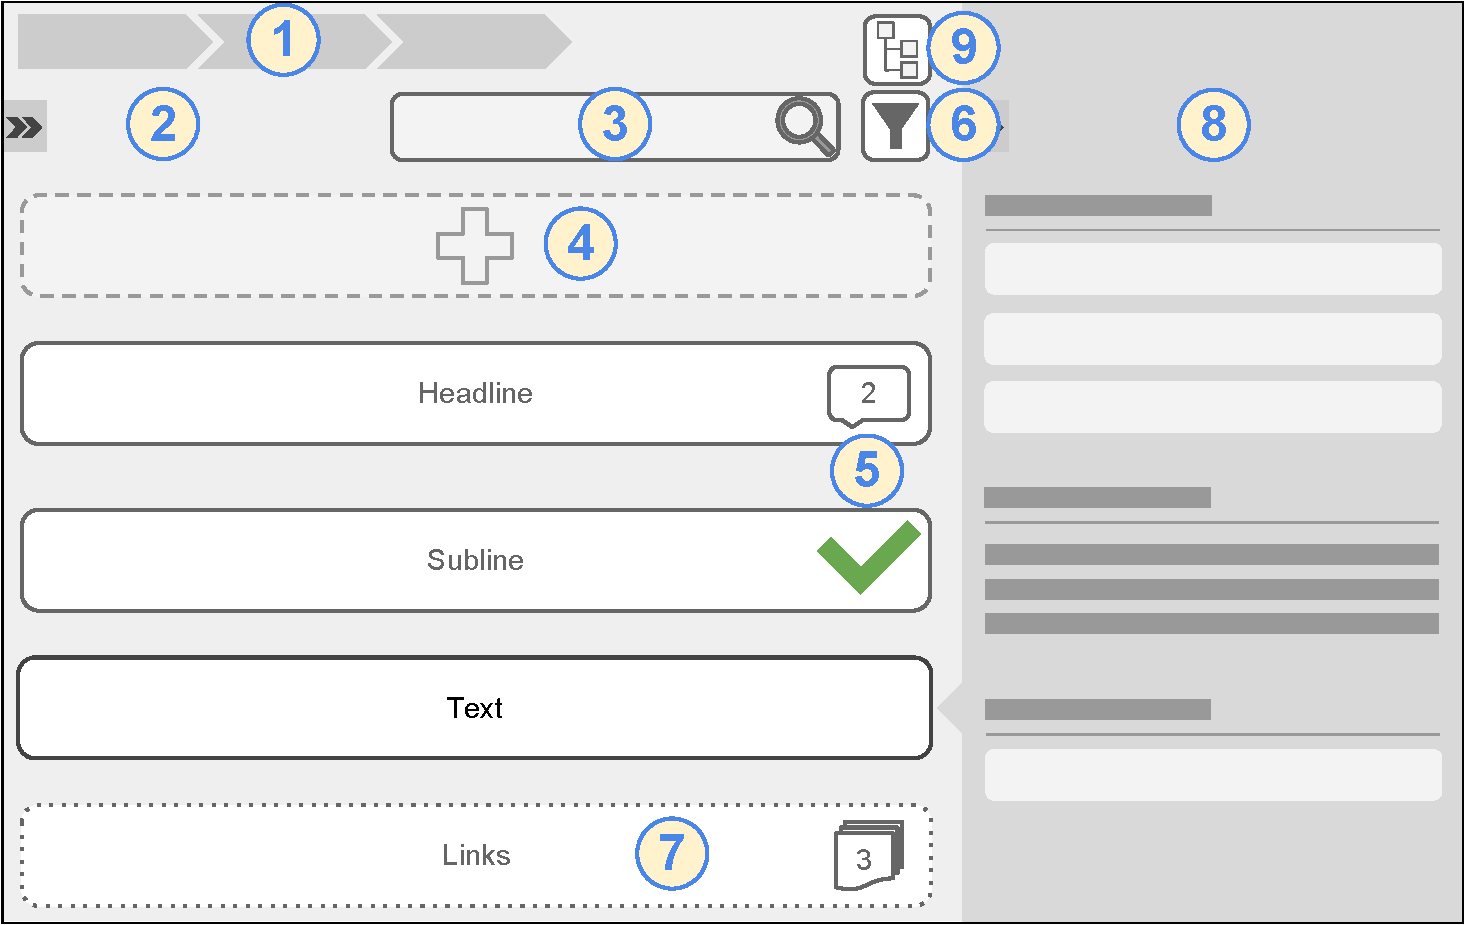
\includegraphics[width=0.95\textwidth]{media/GUIProduktstruktur.pdf}
\captionof{figure}{GUI zum Bearbeiten der Produktstruktur}\label{chart:gui-produktstruktur}
\end{center}

Abbildung~\ref{chart:gui-produktstruktur} zeigt die Darstellung des GUIs zur Bearbeitung der Produktstruktur. Über die Breadcrumb-Navigation \ball{1}, die die aktuelle Position in der Projekthierarchie zeigt, ist eine Orientierung auch ohne das eingeklappte Projektmenü möglich. Über eine Schaltfläche lassen sich alle Container aber der aktuellen Hierarchiebene aufklappen, so ist können umfangreiche Änderungen an vielen Elementen gleichzeitig vorgenommen werden, ohne dass man sich durch die verschiedenen Ebenen \typoquotes{hangeln} muss. Im Inhaltsbereich \ball{2} werden die auf der aktuellen Ebene befindlichen Inhalts-Elemente, Textbausteine und Container, angezeigt. Die Darstellung erfolgt in eine kompakten Weise, die einen schnellen Überblick über die Inhalte bietet ohne viel Scrollen zu müssen. Die einzelnen Inhalts-Elemente können mit Drag\&Drop in ihrere Reihenfolge angepasst werden. Über das Suchfeld \ball{3} können die angezeigten Elemente gefiltert werden. Über eine Schaltfläche \ball{4} können neue Inhalts-Elemente erstellt werden. Zusatzinformationen wie der Typ, der Status, Kommentare oder ähnliche können auch verwendet werden, um die Inhalte auf der Seite zu filtern, z.B. um nur die Element anzuzeigen, für die noch die Inhalte fehlen \ball{5}. Durch Klick auf einen Container \ball{6} gelangt man eine Ebene tiefer, in diesen Conatiner hinein. Das Icon gibt die Anzahl der untergeordneten Element an. In der Spalte für die Kontext-Information \ball{7} werden Detailinformation zum aktuell ausgewählten Element dargestellt, die an die eingestellten Ansichts-Art angepasst sind. Hier findet sich auch die Bearbeitungshistorie und die Kommentare zu den Inhalts-Elementen.

Über eine Schaltfläche \ball{8} kann zwischen den vier Ansichten (Definieren~\ref{l:gui-definition}, Texten~\ref{l:gui-texten}, Übersetzen~\ref{l:gui-uebersetzen} und Kontrolle~\ref{l:gui-qs}), die die Inhaltselemente manipulieren, gewechselt werden.

\subsubsection{Texte erstellen}\label{l:gui-texten}

\begin{center}
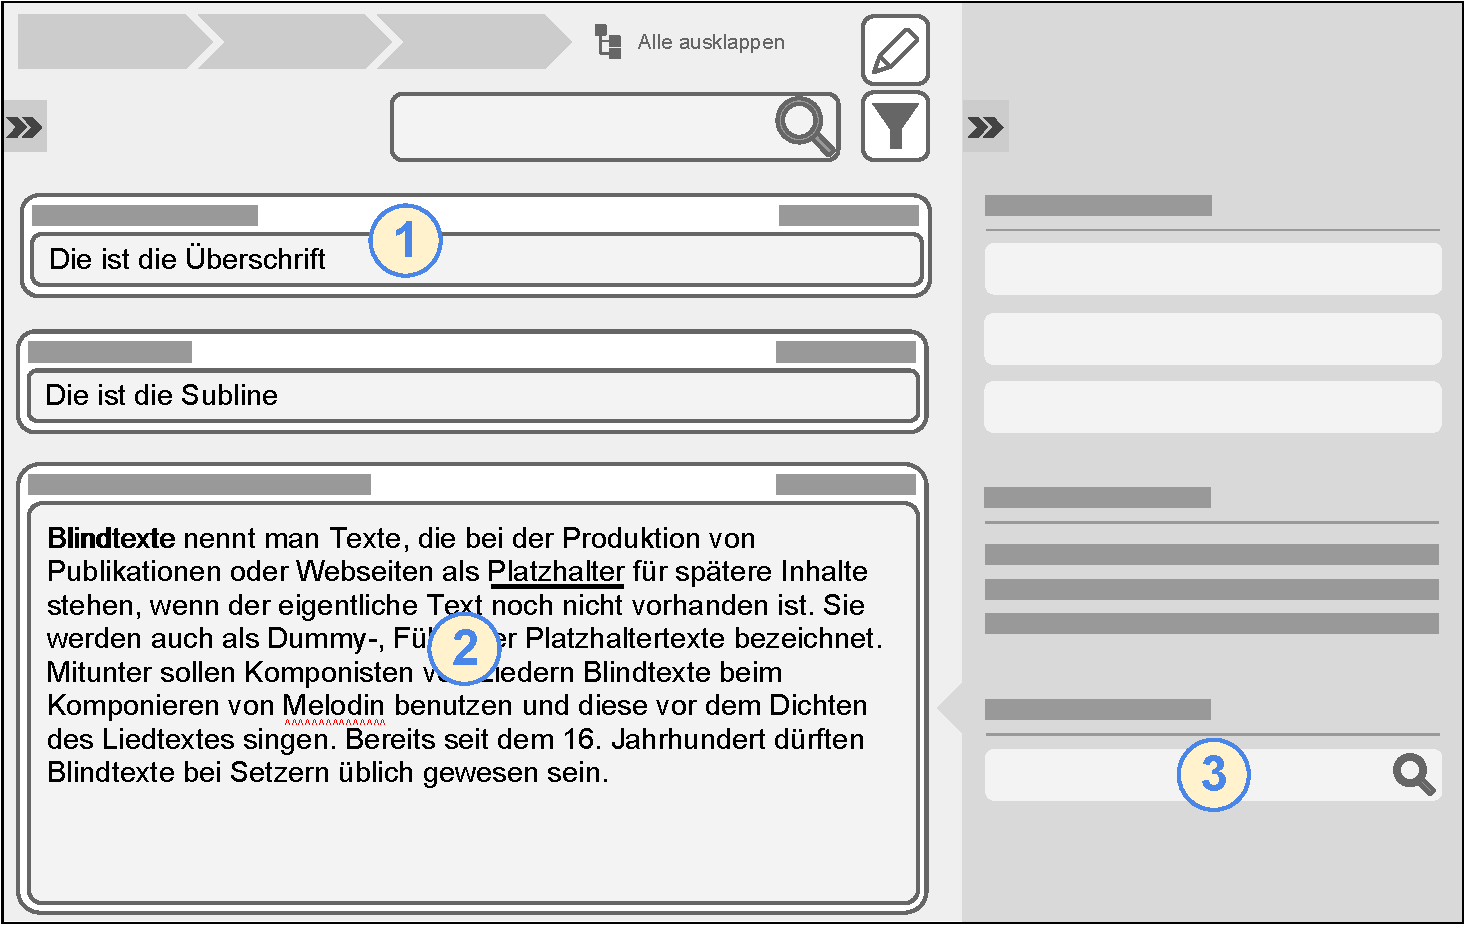
\includegraphics[width=0.95\textwidth]{media/GUITexteerstellen.pdf}
\captionof{figure}{GUI zum Erstellen der Texte}\label{chart:gui-texten}
\end{center}

Abbildung~\ref{chart:gui-texten} zeigt die Darstellung des GUIs zur Bearbeitung der Texte des Produktes. Die Inhaltselemente in der aktuelle Hierarchie werden dabei mit Eingabefeldern für die Inhalte dargestellt \ball{1}. Links über dem Eingabefeld wird die Bezeichnung des Textbausteins angezeigt und rechts darüber Hinweise zu Längebeschränkungen (falls vorhanden) mit Zähler. Während der Eingabe können bereits Auszeichnungen vorgenommen werden, die Schaltflächen dazu, werden eingeblendet, sobald sich der Cursor im Feld befindet. Innerhalb der Kontext-Informationen \ball{3} besteht die Möglichkeit direkt eine Suche zu starten, die Suchergebnisse werden in einem Dialog-Fenster geöffnet. 

\subsubsection{Texte übersetzen}\label{l:gui-uebersetzen}

\begin{center}
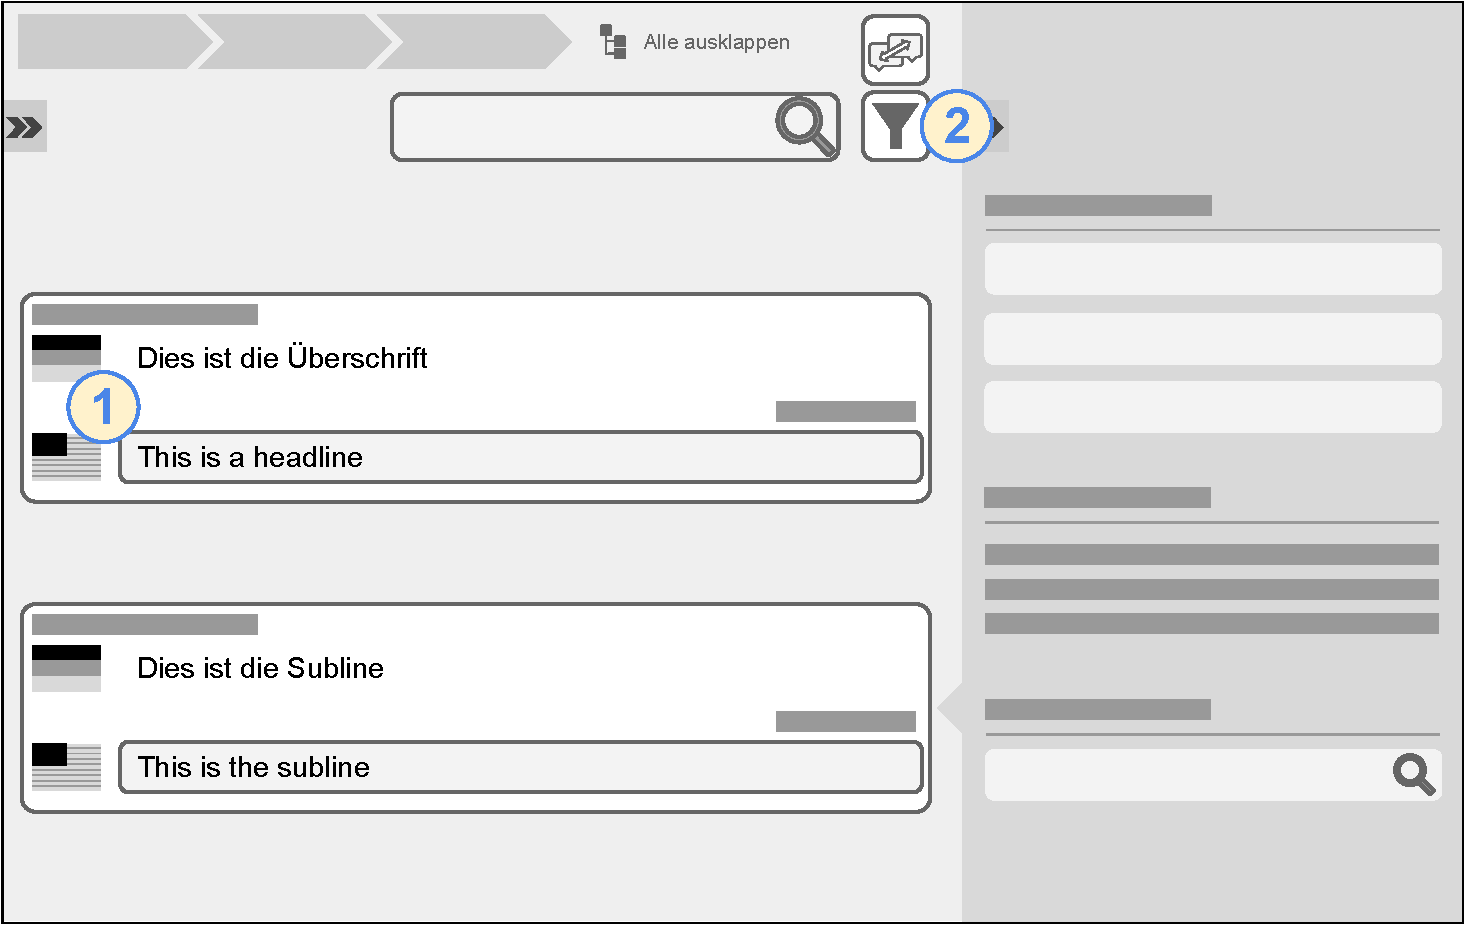
\includegraphics[width=0.95\textwidth]{media/GUITexteuebersetzen.pdf}
\captionof{figure}{GUI zum Übersetzen der Texte}\label{chart:gui-uebersetzen}
\end{center}

Abbildung~\ref{chart:gui-uebersetzen} zeigt die Darstellung des GUIs zur Übersetzung der Texte des Produktes. Hierzu wird der Inhalt des Textbausteines in der Original-Sprache angezeigt und darunter ein Eingabefeld, in dem die Übersetzung eingetragen wird \ball{1}. Über einen Filter-Dialog \ball{2} kann konfiguriert werden, welche Sprachen angezeigt werden sollen.

\subsubsection{Prüfen}\label{l:gui-qs}

\begin{center}
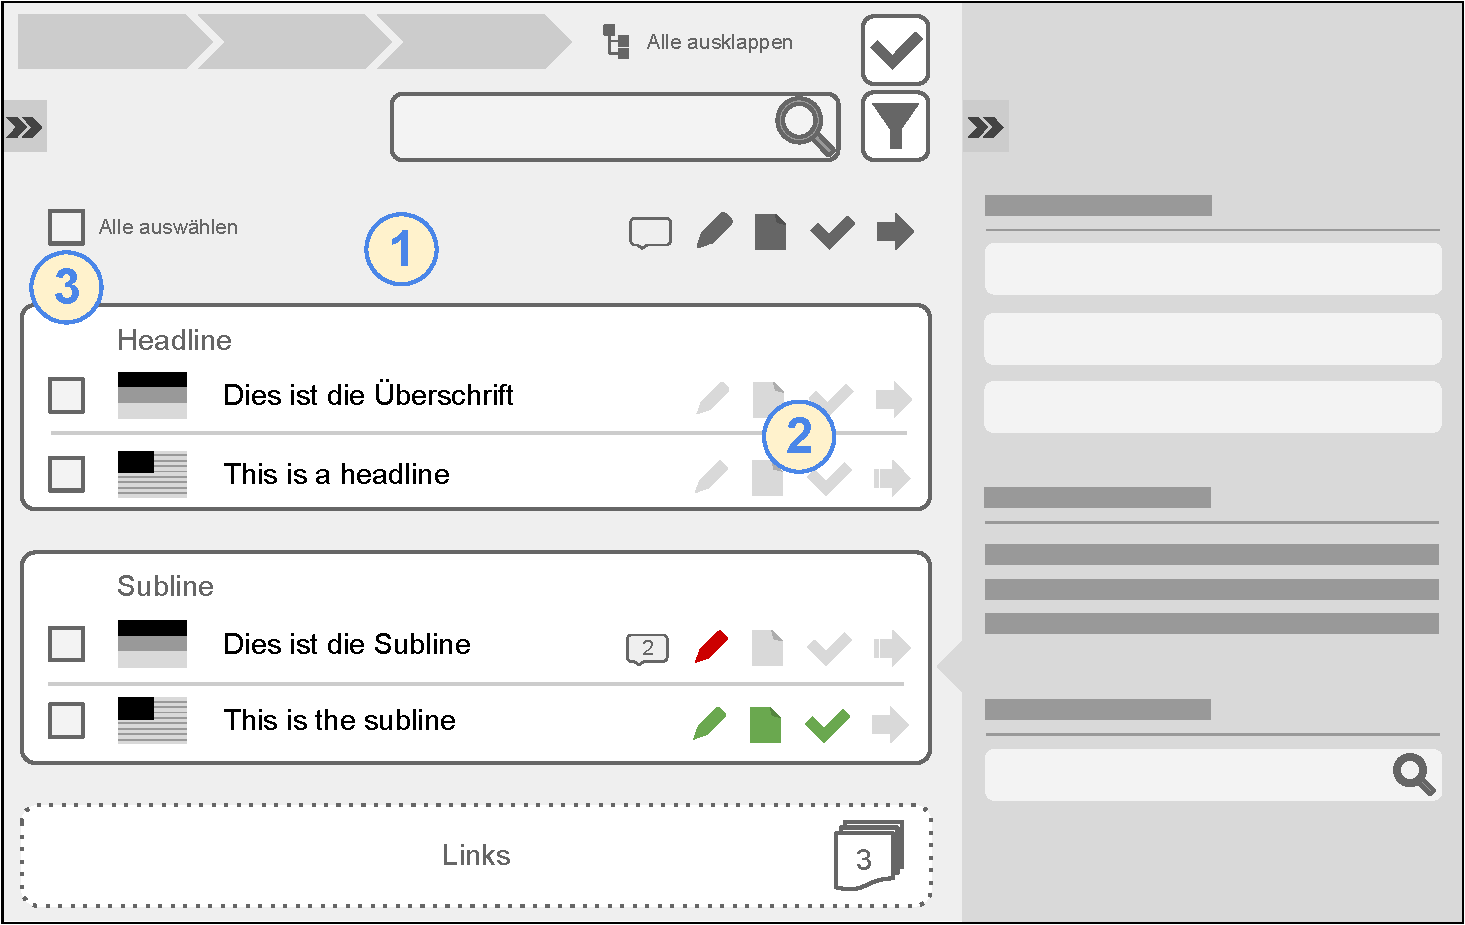
\includegraphics[width=0.95\textwidth]{media/GUIFreigabe.pdf}
\captionof{figure}{GUI zum Überprüfen der Texte}\label{chart:gui-qs}
\end{center}

Abbildung~\ref{chart:gui-qs} zeigt die Darstellung des GUIs zur Kontrolle und Freigabe der Texte des Produktes. In dieser Ansicht werden die verschiedenen Stati der Textbausteine bearbeitet. Hierzu sind die Textbausteine mit ihren Übersetzungen dargestellt \ball{1}. Über die mit Icons markierten Schaltflächen \ball{2} lassen sich die einzelnen Stati direkt setzen. Von links nach rechts sind das: Korrigiert, Geprüft, Freigegeben und Veröffentlicht. Es wird jeweils zwischen \typoquotes{keine Angabe} (grau), \typoquotes{abgelehnt} (rot) und \typoquotes{in Ordnung} (grün) unterschieden. Hier wird auch die Anzahl der hinterlegten Kommentare angezeigt. Zum massenhaften bearbeiten von Stati können mehrere oder alle Elemente über die Checkboxen \ball{3} ausgewählt werden. Über die Status-Icons in der Kopfzeile kann dann der Status für alle ausgewählten Elemente gleichzeitig gesetzt werden.

\subsubsection{Kontext-Informationen}\label{l:gui-kontext}

\begin{center}
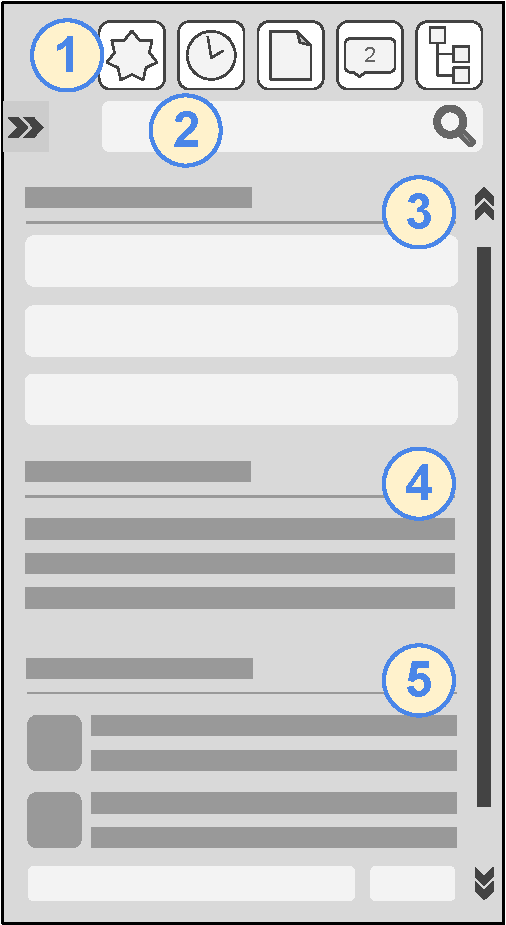
\includegraphics[width=0.35\textwidth]{media/GUIKontext-Informationen.pdf}
\captionof{figure}{Kontext-Informationen}\label{chart:gui-kontext}
\end{center}

Abbildung~\ref{chart:gui-kontext} zeigt die Darstellung des GUIs zur Anzeige und Bearbeitung der Kontext-Informationen. Der Inhalt der Ansicht ist an die jeweilige Operation angepasst. Im oberen Bereich kann zwischen verschiedenen Kontextinformationen zu dem jeweiligen Inhalt umgeschaltet werden \ball{1} (v.l.n.r): 

\begin{enumerate}\itemsep -5pt
\item Neues: Listet die neuesten Informationen aus den vier Bereichen und den aktuellen Status.
\item Änderungshistorie: Zeigt die vergangenen Änderungen an, mit der Möglichkeit, diese zu kommentieren und zurückzunehmen.
\item Material: Zeigt hinterlegte Materialien an. Dabei handelt es sich um Dateien und Freitext-Notizen.
\item Kommentare: Zeigt die Kommentare an.
\item Struktur: Zeigt Informationen zur Struktur innerhalb des Produktes, wie z.B. die Attribute, an.
\end{enumerate}

Über das Suchfeld \ball{2} lässt sich die aktuellen Ansicht filtern. In den Kontextinformation findet sich direkter Zugang zu Informationen und Operationen bezogen auf den aktuellen Inhalt. Die Inhalte lassen sich über Formulare \ball{3} direkt bearbeiten, Notizen und Dateien werden angezeigt \ball{4} und der Diksussion mithilfe der Kommentarfunktion ist möglich \ball{5}.

\subsection{Anbindung der GUI an den Server}\label{l:anbindung-gui}

Die in Abbildung~\ref{chart:komponenten}~(S.\pageref{chart:komponenten}) \emph{gelb} eingezeichneten Komponenten zeigen den Aufbau eines browserbasierten GUIs. Mittlerweile ist es üblich, klassische Paradigmen aus der Softwarentwicklung auch in browserbasierten Anwendung zu verwenden. Dementsprechend wird die GUI in Form einer MVC-Anwendung implementiert. Die Kommunikation mit dem Server wird in einer eigenen Komponente, dem \emph{API-Adapter}, gekapselt, die über die REST-Schnittstelle JSON-Daten mit dem Server austauscht. Die Repräsentation der Domänendaten erfolgt dabei mithilfe von entsprechenden \emph{Models}, die durch die \emph{Controller} mit den \emph{Views} verbunden werden. Die Models sind nicht zwangsläufig mit den Models auf der Serverseite identisch sondern können Aggregationen sein, oder nur Teile der Daten abbilden, sie orientieren sich an der öffentlichen API des Servers, die nicht zwingenderweise die interenen Models 1:1 nach außen weiterreicht. Views sind einzelne Bestandteile einer Ansicht. So lassen sich individuelle Bereiche der Darstellung leicht aktualisieren, ohne die ganze Seite neu laden zu müssen -- in \cite[S.1--5 und S.65--72]{maccaw2011javascript} ist dieses Prinzip ausführlich erläutert.

\subsection{Entwurf des Anwendungsservers}\label{l:entwurf-server}

In Abbildung~\ref{chart:komponenten}~(S.\pageref{chart:komponenten}) finden sich die Komponenten des Servers grau eingefärbt. 

\subsubsection{API, Cronjobs, CLI, …}

\subsubsection{Controller}

\subsubsection{Models}

\subsubsection{Dependency-Injection-Container}

\subsubsection{Workflow}

\subsubsection{Service-Adapter}

\subsubsection{Persistenz, ORM}

\subsubsection{Jobs}

\subsubsection{Import/Export \& Benachrichtigung}



\subsection{Domänenmodell}\label{l:domänenmodell}

\begin{center}
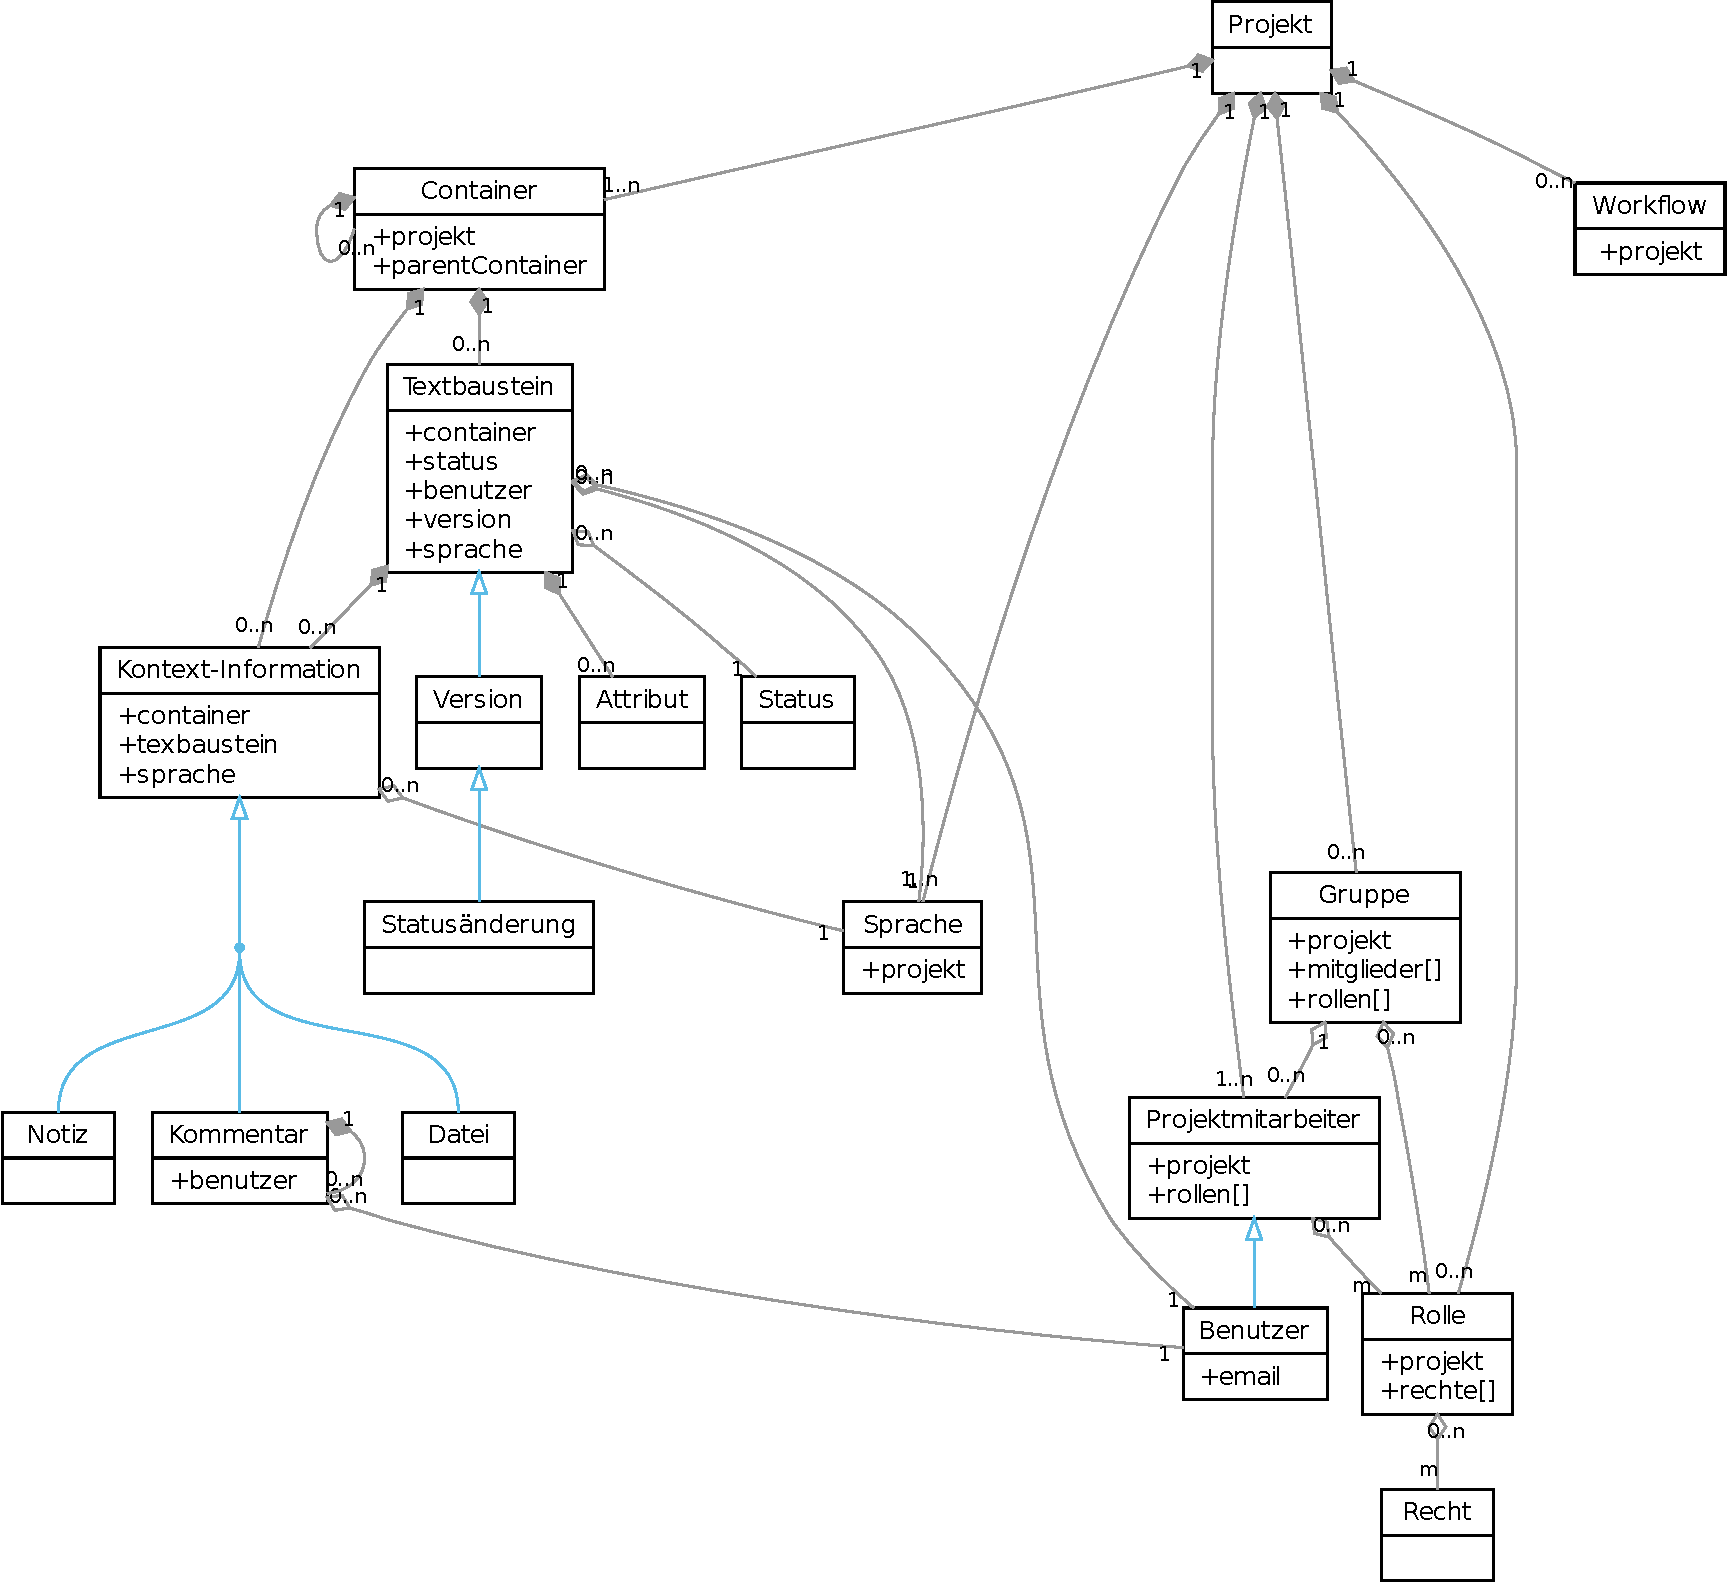
\includegraphics[width=\textwidth]{media/domain.pdf}
\captionof{figure}{Domänenmodell}\label{chart:domain}
\end{center}

Aus den vorangegangenen Überlegungen zur Anwendung und zum Workflow lässt sich ein Domänenmodell extrahieren, die einzelnen logischen Objekte innerhalb der Anwendung beschreibt, mit deren Hilfe alle Operationen abgebildet werden. Abbildung~\ref{chart:domain} zeigt das Modell in der Übersicht, dass die sich im Entwurf der Anwendung in deren Implementierung im Prototypen widerspiegelt.

\textsf{\textbf{Attribut}}\\Beschreibt die Attribute eines Textbausteins.

\textsf{\textbf{Benutzer}}\\Repräsentiert einen Benutzer des Systems

\textsf{\textbf{Container}}\\Containern dienen zur hierarchischen Organisation der Texte innerhalb des Projektes. Containern können weitere Container und Texte enthalten. Eine Container ohne übergeordneten Container befindet sich auf der obersten Ebene. Es kann mehrere Containern auf der obersten Ebene geben.

\textsf{\textbf{Gruppe}}\\Mitarbeiter können in Gruppen zusammengefasst werden. Dies erleichtert die Konfiguration des Workflows und der Rechte.

\textsf{\textbf{Kommentare}}\\Kommentare enthalten Hinweise und Fragen zu einzelnen Texten und Texbausteinen.

\textsf{\textbf{Kontext-Information}}\\Projektspezifische Kontext-Informationen lassen sich hinterlegen und Textbausteinen und Containern zuordnen.

\textsf{\textbf{Projekt}}\\Projekte bildet den Rahmen für alle Texte eines einzelnen Produktes.

\textsf{\textbf{Projektmitarbeiter}}\\Gestattet einem Benutzer die Mitarbeit an einem Projekt und legt dabei fest, welche Rechte dem Benutzer für das Projekt zustehen.

\textsf{\textbf{Recht}}\\Beschreibt ein Recht, eine Operation auf einem Objekt auszuführen.

\textsf{\textbf{Rolle}}\\Beschreibt die verschiedenen Rollen innerhalb der Anwendung. Die Rechte der Rollen sind durch die Zuordnung von Benutzern zu Projekten durch den Projektmitarbeiter immer an das jeweilige Projekt gebunden.

\textsf{\textbf{Sprache}}\\Die Texte jedes Projekts liegen in einer oder mehreren Sprachen vor.

\textsf{\textbf{Status}}\\Beschreibt die verschiedenen Zustände eines Textbausteins (vgl. Abschnitt \ref{l:konzept-workflow-status} · S.\pageref{l:konzept-workflow-status}).

\begin{enumerate}\itemsep -5pt
\item \texttt{Neu}, Textbaustein erzeugt
\item \texttt{Leer}, Textbaustein definiert
\item \texttt{Befüllt}, Textbaustein mit Inhalt befüllt
\item \texttt{Korrigiert}, Orthografie geprüft
\item \texttt{Geprüft}, Inhalt geprüft (Qualitätsicherung)
\item \texttt{Freigegeben}, durch Kunden freigegeben
\item \texttt{Veröffentlicht}, in Produkt übernommen
\end{enumerate}

\textsf{\textbf{Statusänderung}}\\Beschreibt eine Änderung eines Status durch einen Benutzer, z.B. durch Freigabe oder Überprüfung.

\textsf{\textbf{Textbaustein}}\\Beschreibt einen einzelnen Textbaustein.

\textsf{\textbf{Version}}\\Beschreibt eine Version des Inhalts eines Textbausteins.

\textsf{\textbf{Workflow}}\\Beschreibt einen projektspezifischen Workflow.


\pagebreak